\section{Stromspiegel}
In diesem Versuch soll der Stromspiegel aus den vorbereitenden Aufgaben
aufgebaut und vermessen werden. Verwenden Sie f\"ur diesen Versuch den Transistor
CD4007 mit einer symmetrische Spannungsversorgung von $\pm$5 V, da dieser f\"ur die
folgenden Versuche wieder ben\"otigt wird.
\subsection{Experimentelle Durchf\"uhrung}
Es wurde die Schaltung aus Abbildung 1 auf dem Steckbrett aufgebaut, dabei wurde der Transistor CD4007 verwendet. F\"ur den ersten Mosfet wurde das Kabel zum Gate auf Pinn 3, zum Source auf Pinn 4 und zum Drain auf Pinn 4 des Transistors eingesteckt. F\"ur den zweiten Mosfet wurde das Kabel zum Gate auf Pinn 6, zum Source auf Pinn 7 und zum Drain auf Pinn 8 eingesteckt. Die jeweiligen Gates (Pinn 3 und Pinn 6) wurden mit einem Kabel verbunden. Als erstes wurde der Referenzstrom sowie der Ausgangsstrom des Stromspiegels gemessen. Danach wurde die Gate-Source Spannung und die Drain-Source Spannung von Transistor M2 vermessen. Im letzten Teil dieses Versuchs wurde ein 20~$k \Omega$ Potentiometer anstelle von R2 eingesetzt und so variiert, dass sich die Spannungen U$_{DS}$ von M2 wie in Tabelle 1 einstellen.
\begin{figure}[!ht]
\begin{center}
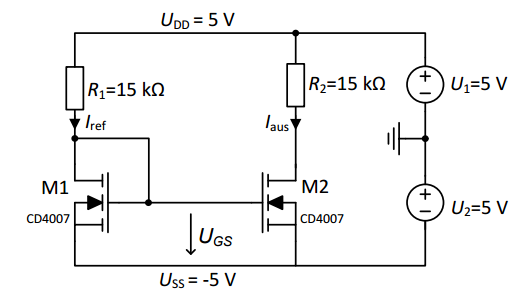
\includegraphics[scale=0.7]{Stromspiegel}
\caption{Stromspiegel}
\end{center}
\end{figure}
\clearpage
\subsection{Ergebnisse und Diskussion}
\begin{figure}[!h]
\begin{center}

\includegraphics[scale=0.8]{Text}
\end{center}
\end{figure}
\begin{figure}[!h]
\begin{center}
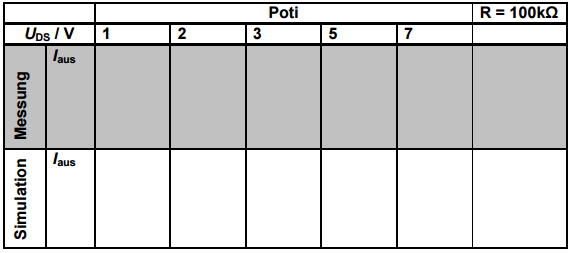
\includegraphics[scale=0.8]{Tabelle1}
\end{center}
\end{figure}
\begin{figure}[!h]
\begin{center}
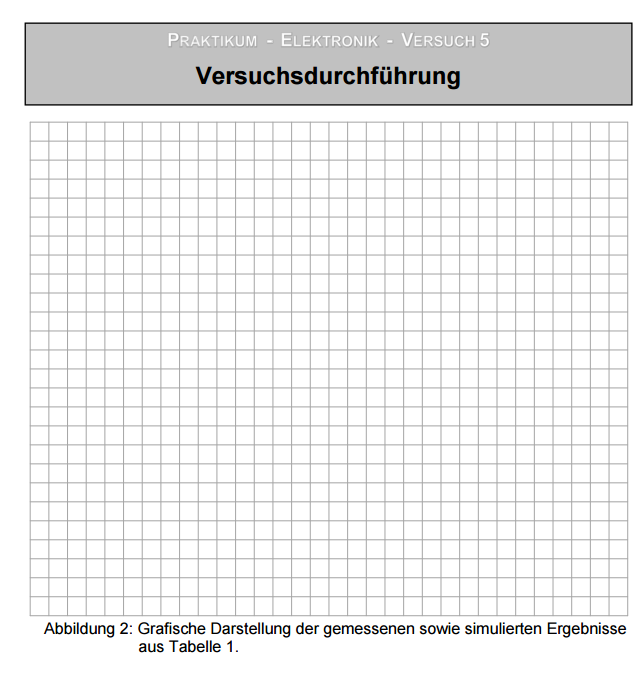
\includegraphics[scale=0.8]{Graph1}
\end{center}
\end{figure}
\clearpage
